\section{Bakti Qilan Mufid}
\subsection{Soal 1}
Buatlah fungsi (file terpisah/library dengan nama \verb|NPM_realtime.py|) untuk mendapatkan data langsung dari arduino

\lstinputlisting[firstline=9, lastline=16]{src/5/1174083/Praktek/1174083_realtime.py}
\begin{figure}[ht!]
	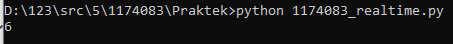
\includegraphics[width=5cm]{figures/5/1174083/Praktek/1.png}
	\centering
	\caption{Membaca Serial tanpa loop}
\end{figure}

\subsection{Soal 2}
Buatlah fungsi (file terpisah/library dengan nama \verb|NPM_save.py|) untuk mendapatkan data langsung dari arduino dengan looping

\lstinputlisting[firstline=10, lastline=18]{src/5/1174083/Praktek/1174083_save.py}


\subsection{Soal 3}
Buatlah fungsi (file terpisah/library dengan nama \verb|NPM_realtime.py|) untuk mendapatkan data dari arduino dan langsung ditulis kedalam file csv
\lstinputlisting[caption="Kode python",firstline=18, lastline=26]{src/5/1174083/Praktek/1174083_realtime.py}
\lstinputlisting[caption="Data yang telah ditulis ke file csv",firstline=0, lastline=10]{src/5/1174083/Praktek/1174083.csv}



\subsection{Soal 4}
Buatlah fungsi (file terpisah/library dengan nama \verb|NPM_csv.py|) untuk membaca file csv hasil arduino dan mengembalikan ke fungsi

\lstinputlisting[firstline=10, lastline=18]{src/5/1174083/Praktek/1174083_csv.py}

\subsection{Ketrampilan Penanganan Error}
Tuliskan peringatan error yang didapat dari mengerjakan praktek ketiga ini, dan jelaskan cara penanganan error tersebut. dan Buatlah satu fungsi yang menggunakan gunakan try except untuk menanggulangi error tersebut.
\begin{itemize}
\item Syntax Errors

Syntax Errors adalah kesalahan pada penulisan syntax atau kode. Solusinya adalah memperbaiki penulisan syntax atau kode

\item Zero Division Error

ZeroDivisonError adalah exceptions yang terjadi saat eksekusi program menghasilkan perhitungan matematika pembagian dengan angka nol (0). Solusinya adalah tidak membagi suatu yang hasilnya nol.

\item Name Error

NameError adalah exception saat kode melakukan eksekusi terhadap local name atau global name yang tidak terdefinisi atau tidak ada. Solusinya adalah memastikan variabel atau function yang akan dipanggil ada didalam program atau tidak salah mengetikannya.

\item Type Error

TypeError adalah exception saat melakukan eksekusi terhadap suatu operasi atau fungsi dengan type object yang tidak sesuai. Solusinya adalah mengkoversi varibelnya sesuai dengan tipe data sesuai dengan yang akan digunakan.

\end{itemize}
\lstinputlisting[firstline=7, lastline=22]{src/5/1174083/Praktek/1174083_error.py}